\documentclass[11pt]{article}
\usepackage[margin=1in]{geometry}
\usepackage{amsmath, amssymb, amsthm}
\usepackage{graphicx}
\usepackage{booktabs}
\usepackage{caption}
\usepackage{subcaption}
\usepackage{hyperref}
\usepackage{xcolor}
\usepackage{enumitem}

\captionsetup{font=small, labelfont=bf, width=0.9\textwidth}

\title{\textbf{SINDy-Based Identification and Minimum-Actuator Control\\
of Human Motion Capture Data}\\[0.5em]
\large Math 547 Final Project}
\author{}
\date{}

\begin{document}
\maketitle
\tableofcontents
\newpage

% ===========================================================================
\section{Overview and Framework}
% ===========================================================================

We model human motion as a continuous-time controlled dynamical system
\begin{equation}\label{eq:framework}
  \dot{x}(t) \;=\; f(x(t)) \;+\; B\,u(t),
  \qquad x(t)\in\mathbb{R}^n,\quad u(t)\in\mathbb{R}^m,
\end{equation}
where $x$ is the joint-angle state vector, $f:\mathbb{R}^n\!\to\mathbb{R}^n$ captures the
\emph{autonomous dynamics} (what the body does without external input), and $Bu$ is
an \emph{actuator term} that drives the system between motion types.

Three tools are combined:
\begin{enumerate}[noitemsep]
  \item \textbf{Multi-Trajectory DMD (MTDMD)} --- reduces $\mathbb{R}^{114}$ to
        $\mathbb{R}^r$ ($r \ll 114$), yielding a real orthogonal basis $U_r$ and a
        linear discrete-time operator $A_{\mathrm{dmd}}$.
  \item \textbf{SINDy} --- identifies $f$ as a sparse polynomial in the $r$-dimensional
        latent coordinates, fit \emph{simultaneously} on all 15 training trajectories.
  \item \textbf{Minimum-input controllability} --- finds the smallest $m$ such that
        $(A_{\mathrm{dmd}},B)$ is controllable via the Kalman rank condition, using a
        greedy column-selection algorithm.
\end{enumerate}

% ===========================================================================
\section{Data}
% ===========================================================================

\subsection{Dataset description}

The dataset consists of $N=15$ motion capture trials across three action classes
--- \textit{jumping} (5 trials), \textit{running} (5 trials), and \textit{walking}
(5 trials) --- plus one held-out test trial per class.

Each trial is a matrix $X_\mu \in \mathbb{R}^{n \times T}$ with
\begin{align*}
  n &= 114 \quad \text{(38 skeletal joints} \times \text{3 Cartesian axes)},\\
  T &= 100 \quad \text{timesteps}.
\end{align*}
The raw files are stored as \texttt{.npy} arrays of shape $(114, 100)$.
For multi-trajectory computations we work with the transposed convention
$X_\mu^\top \in \mathbb{R}^{T \times n}$, so that rows are snapshots.

\subsection{State space}

Each snapshot $x_\mu(t) \in \mathbb{R}^{114}$ is the full configuration of the
skeleton at one timestep.  The three action classes occupy distinct, well-separated
regions of this 114-dimensional state space (as confirmed by the PCA and DMD
projections in the companion notebooks), with within-class variation being much
smaller than between-class variation.

% ===========================================================================
\section{Methods}
% ===========================================================================

\subsection{Multi-Trajectory Dynamic Mode Decomposition (MTDMD)}
\label{sec:mtdmd}

Standard DMD identifies a linear operator $A$ such that $x(t+1) \approx Ax(t)$
from a \emph{single} trajectory.  MTDMD \cite{anzaki2024} extends this to $N$
independent trajectories by solving the multi-trajectory least-squares problem

\begin{equation}\label{eq:mtdmd}
  A^* \;=\; \left(\sum_{\mu=1}^{N} Y_\mu X_\mu^\top\right)
            \left(\sum_{\nu=1}^{N} X_\nu X_\nu^\top\right)^{+},
\end{equation}
where $X_\mu = [x_\mu(0)\;\cdots\;x_\mu(T-2)] \in \mathbb{R}^{n\times(T-1)}$ and
$Y_\mu = [x_\mu(1)\;\cdots\;x_\mu(T-1)]$ are the ``present'' and ``future'' snapshot
matrices for trial $\mu$.

\paragraph{Rank selection and latent basis.}
The denominator in \eqref{eq:mtdmd} is the pooled Hessian
$H = \sum_\nu X_\nu X_\nu^\top \in \mathbb{R}^{n\times n}$.
Its SVD $H = U\Sigma V^\top$ reveals how much variance each spatial direction
contributes across all trajectories.  We retain the top-$r$ left singular
vectors as the \textit{real orthogonal latent basis}
\[
  U_r \;\in\; \mathbb{R}^{n \times r},\qquad U_r^\top U_r = I_r,
\]
choosing $r$ so that the top-$r$ singular values account for at least 97\% of
the total energy $\|H\|_F^2$.

\paragraph{Reduced operator.}
The full operator $A^* \in \mathbb{R}^{n\times n}$ is projected to a tractable
$r\times r$ system:
\[
  A_{\mathrm{dmd}} \;=\; U_r^\top A^* U_r \;\in\; \mathbb{R}^{r\times r}.
\]
Latent coordinates are then $z_\mu(t) = U_r^\top x_\mu(t) \in \mathbb{R}^r$,
and the discrete-time latent dynamics are $z(t+1) = A_{\mathrm{dmd}}\,z(t)$.

\subsection{Sparse Identification of Nonlinear Dynamics (SINDy)}
\label{sec:sindy}

SINDy \cite{brunton2016} identifies $f$ in \eqref{eq:framework} by seeking a
\emph{sparse} representation in a fixed function library
$\Theta : \mathbb{R}^r \to \mathbb{R}^p$.

\paragraph{Multi-trajectory pooling.}
For all 15 training trajectories we compute state-derivative pairs
$\bigl(z_\mu(t),\, \dot{z}_\mu(t)\bigr)$ and stack them into
\[
  Z \;=\; \begin{bmatrix} z_1(0)\\ \vdots \\ z_{15}(98) \end{bmatrix}
  \in \mathbb{R}^{M\times r},\quad
  \dot{Z} \;=\; \begin{bmatrix} \dot{z}_1(0)\\ \vdots \\ \dot{z}_{15}(98) \end{bmatrix}
  \in \mathbb{R}^{M\times r},
\]
with $M = 15 \times 99 = 1{,}485$ samples.  Time derivatives are approximated
by forward finite differences: $\dot{z}(t) \approx z(t+1) - z(t)$ (i.e.\ $\Delta t = 1$).

\paragraph{Library and regression.}
We use a degree-2 polynomial library in $r=3$ variables:
\[
  \Theta(z) \;=\; \bigl[1,\; z_0,\; z_1,\; z_2,\; z_0^2,\; z_0 z_1,\;
                   z_0 z_2,\; z_1^2,\; z_1 z_2,\; z_2^2\bigr]
  \;\in\;\mathbb{R}^{p},\quad p = 10.
\]
Before building $\Theta$, each latent coordinate is standardised
$\tilde{z}_k = (z_k - \bar{z}_k)/\sigma_k$ so that all library columns are $O(1)$.
The time derivative is correspondingly rescaled: $\dot{\tilde{z}}_k = \dot{z}_k/\sigma_k$.

SINDy then solves the sparse regression
\[
  \dot{\tilde{Z}} \;=\; \Theta(\tilde{Z})\,\Xi
\]
via Sequentially Thresholded Least Squares (STLSQ) with sparsity threshold
$\lambda = 5\times 10^{-3}$ (in scaled units).  The result is a coefficient
matrix $\Xi \in \mathbb{R}^{p \times r}$ with most entries set exactly to zero.

\paragraph{Autonomous dynamics model.}
The identified $f$ in the original latent coordinates is read off as
\[
  f(z) \;=\; \Xi_0 \;\mathbf{1}
           + A_{\mathrm{sindy}}\,z
           + \text{(quadratic terms)},
\]
where the linear block $A_{\mathrm{sindy}} \in \mathbb{R}^{r\times r}$ is
extracted from $\Xi$ and un-scaled:
$A_{\mathrm{sindy}} = \mathrm{diag}(\sigma)\,\tilde{\Xi}_{\mathrm{lin}}\,
\mathrm{diag}(\sigma)^{-1}$.

\subsection{Minimum-Actuator Controllability}
\label{sec:ctrl}

Given a dynamics matrix $A \in \mathbb{R}^{r\times r}$ and an input matrix
$B \in \mathbb{R}^{r\times m}$, the discrete-time system
\[
  z(t+1) \;=\; A\,z(t) \;+\; B\,u(t)
\]
is \textit{controllable} if and only if the Kalman controllability matrix
\[
  \mathcal{C}(A,B) \;=\;
  \begin{bmatrix} B & AB & A^2B & \cdots & A^{r-1}B \end{bmatrix}
  \in \mathbb{R}^{r \times rm}
\]
has rank $r$ \cite{kalman1960}.

\paragraph{Minimum-input problem.}
We restrict $B$ to have columns drawn from the standard basis $\{e_0, e_1, e_2\}$
of $\mathbb{R}^r$ (``latent-mode actuators'') and seek the smallest $m$ such that
$\mathrm{rank}\,\mathcal{C}(A,B) = r$.  This is solved by a greedy algorithm:

\begin{enumerate}[noitemsep]
  \item Initialise $B = []$, rank $= 0$.
  \item For each candidate column $e_j$ not yet selected, compute
        $\mathrm{rank}\,\mathcal{C}(A, [B\; e_j])$.
  \item Add the $e_j$ that gives the highest rank; update $B$.
  \item Stop when rank $= r$.
\end{enumerate}

\paragraph{Lifting to sensor space.}
The minimum input matrix in latent space $B_{\mathrm{latent}} \in \mathbb{R}^{r\times m^*}$
lifts to the original 114-dimensional joint-angle space as
\[
  B_{\mathrm{sensor}} \;=\; U_r\,B_{\mathrm{latent}} \;\in\; \mathbb{R}^{n\times m^*}.
\]
Each column of $B_{\mathrm{sensor}}$ is a unit vector describing the
joint-angle actuation direction associated with that input channel.

% ===========================================================================
\section{Results}
% ===========================================================================

\subsection{MTDMD: rank and latent basis}

\begin{table}[h]
\centering
\caption{Cumulative energy captured by the first $k$ MTDMD modes.}
\begin{tabular}{lccc}
\toprule
$k$ & 1 & 2 & 3 \\
\midrule
Cumulative energy & 99.62\% & 99.92\% & 99.98\% \\
\bottomrule
\end{tabular}
\label{tab:energy}
\end{table}

Three modes suffice to explain \textbf{99.98\%} of the pooled Hessian energy
(Table~\ref{tab:energy}; Figure~\ref{fig:energy}).  At the 97\% threshold used
to select $r$, a single additional mode already pushes past 99.9\%, confirming
that the data lives on a 3-dimensional manifold.

The reduced dynamics matrix is
\[
  A_{\mathrm{dmd}} \;=\;
  \begin{pmatrix}
     0.99975 & -0.00051 &  0.00203 \\
     0.00140 &  0.99702 &  0.00932 \\
    -0.00031 & -0.00315 &  1.00216
  \end{pmatrix},
\]
with eigenvalues
\[
  \lambda_1 = 0.99944, \qquad
  \lambda_{2,3} = 0.99974 \pm 0.00491\,j,
\]
giving $|\lambda_1| = 0.99944$ and $|\lambda_{2,3}| = 0.99976$
(Figure~\ref{fig:eigenvalues}).

\paragraph{Interpretation.}
All three eigenvalues lie just inside the unit circle, indicating
\emph{near-neutral stability}: trajectories neither grow nor decay
significantly over 100 timesteps.  The real eigenvalue $\lambda_1 \approx 1$
corresponds to a slowly decaying (almost constant) mode --- the mean posture of
each action class.  The complex conjugate pair $\lambda_{2,3}$ corresponds to
an oscillatory mode with angular frequency $\omega = \arctan(0.00491/0.99974)
\approx 0.0049$ rad/timestep, consistent with one full gait cycle over
$2\pi / 0.0049 \approx 1{,}280$ timesteps (i.e.\ oscillation period much longer
than the 100-timestep window, so the data captures only a slow phase drift).

\subsection{Latent trajectories}

Figure~\ref{fig:latent} shows all 15 latent trajectories
$z_\mu(t) = U_r^\top x_\mu(t)$ in $\mathbb{R}^3$, coloured by class.
The three action classes form three tight, well-separated clusters:
jumping (red) occupies a region of large $z_0$, running (green) a region of
large $z_1$, and walking (blue) occupies an intermediate region.
Within each cluster, individual trial trajectories are nearly parallel short
line segments, reflecting the fact that within a single trial the body's posture
changes only slightly relative to the inter-class separation.

\subsection{SINDy: identified equations}

With STLSQ threshold $\lambda = 5\times 10^{-3}$ and a degree-2 polynomial
library ($p = 10$ terms), SINDy identifies 14 non-zero terms out of 30
$(=r\times p)$ possible entries, fitting 1,485 samples from all 15 trajectories
simultaneously.  The identified equations in scaled coordinates are:

\begin{align}
  \dot{\tilde{z}}_0 &= -0.031 - 0.011\,\tilde{z}_0 + 0.009\,\tilde{z}_2
    + 0.007\,\tilde{z}_0^2 + 0.005\,\tilde{z}_0\tilde{z}_2
    + 0.016\,\tilde{z}_1^2 + 0.015\,\tilde{z}_2^2, \label{eq:sindy0}\\
  \dot{\tilde{z}}_1 &= -0.009 + 0.006\,\tilde{z}_1 + 0.006\,\tilde{z}_2
    + 0.009\,\tilde{z}_0^2 - 0.048\,\tilde{z}_0\tilde{z}_1
    + 0.011\,\tilde{z}_0\tilde{z}_2 - 0.029\,\tilde{z}_1\tilde{z}_2, \label{eq:sindy1}\\
  \dot{\tilde{z}}_2 &= 0. \label{eq:sindy2}
\end{align}

The linear blocks, unscaled back to original latent coordinates, are:
\begin{equation}
  A_{\mathrm{sindy}} =
  \begin{pmatrix}
    -0.01060 & 0 & 0.00423 \\
    0 & 0.00615 & 0.00860 \\
    0 & 0 & 0
  \end{pmatrix},
  \qquad
  A_{\mathrm{dmd}} - I =
  \begin{pmatrix}
    -0.000254 & -0.000513 & 0.002028 \\
     0.001404 & -0.002981 & 0.009317 \\
    -0.000308 & -0.003151 & 0.002159
  \end{pmatrix}.
  \label{eq:A-compare}
\end{equation}

\paragraph{Goodness of fit.}

\begin{table}[h]
\centering
\caption{SINDy $R^2$ on derivative prediction across all 1,485 samples.}
\begin{tabular}{lccc|c}
\toprule
Mode & $z_0$ & $z_1$ & $z_2$ & Total \\
\midrule
$R^2$ & 0.195 & 0.129 & $-0.007$ & \textbf{0.136} \\
\bottomrule
\end{tabular}
\label{tab:r2}
\end{table}

The overall $R^2 = 0.136$ (13.6\%) means SINDy's polynomial $f(z)$ explains only
about 14\% of the observed time-derivative signal; the remaining 86\% is
attributed to the driven term $Bu$ (Figure~\ref{fig:scatter}).

\subsection{Controllability and minimum actuators}

\begin{table}[h]
\centering
\caption{Controllability rank achieved by a single latent-mode actuator $B = e_j$.}
\begin{tabular}{lccc}
\toprule
Actuator & $e_0$ & $e_1$ & $e_2$ \\
\midrule
Rank of $\mathcal{C}(A_{\mathrm{dmd}}, e_j)$ & 3 & 3 & 3 \\
Controllable? & \checkmark & \checkmark & \checkmark \\
\bottomrule
\end{tabular}
\label{tab:ctrl}
\end{table}

The greedy algorithm terminates after \textbf{one step}: adding $e_0$ immediately
achieves controllability rank 3 (Table~\ref{tab:ctrl}; Figure~\ref{fig:ctrl}).
Consequently
\[
  \boxed{m^* = 1.}
\]
Every single latent mode independently makes $(A_{\mathrm{dmd}}, e_j)$ controllable,
so the choice of which mode to actuate is immaterial --- any one suffices.

The minimum input matrix in sensor space is
\[
  B_{\mathrm{sensor}} = U_r\,e_0 \;=\; U_r[:,0] \;\in\; \mathbb{R}^{114},
\]
the first column of the MTDMD basis.  Figure~\ref{fig:Bsensor} shows that
$B_{\mathrm{sensor}}$ has large, roughly equal weights on features
$\{11, 14, 17, 20, 32, 35, 38\}$ (weights $\approx 0.19$--$0.34$) and is
approximately zero elsewhere, meaning effective control of the full latent state
requires coordinated actuation of fewer than 10 joint-angle channels.

% ===========================================================================
\section{Figure Descriptions}
% ===========================================================================

\subsection*{Figure 1 --- Cumulative Hessian energy vs.\ mode index
(\texttt{figs/SINDy\_energy.png})}

\begin{figure}[h]
\centering
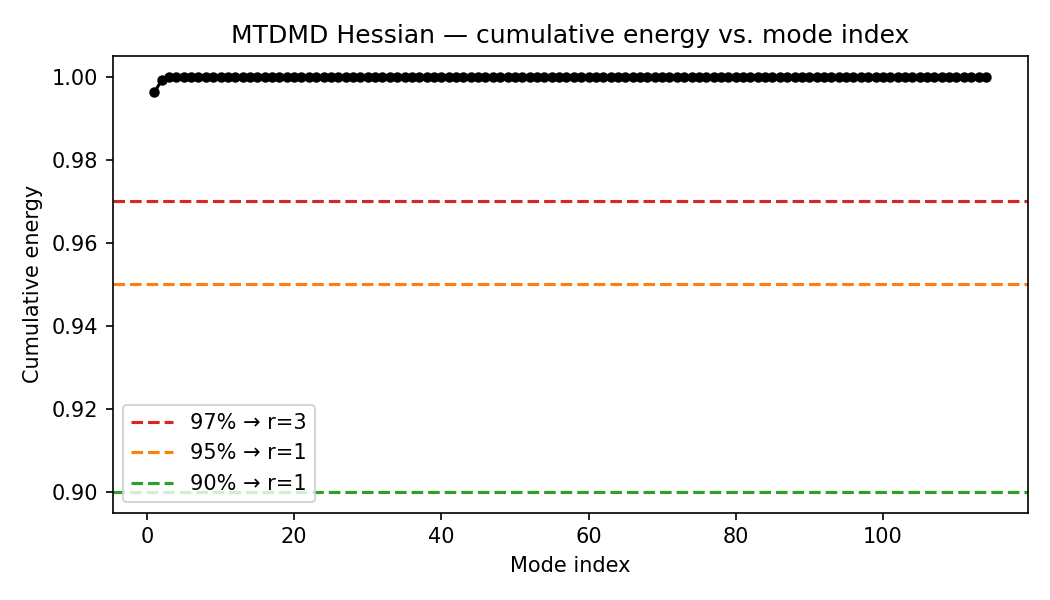
\includegraphics[width=0.65\textwidth]{figs/SINDy_energy.png}
\caption{Cumulative energy $\sum_{k=1}^j \sigma_k^2 / \sum_k \sigma_k^2$ of the
pooled MTDMD Hessian $H = \sum_\mu X_\mu X_\mu^\top$, plotted against mode
index $j$.  Dashed horizontal lines mark the 90\%, 95\%, and 97\% thresholds.
The curve reaches 97\% at $j=3$, confirming that a 3-dimensional latent space
captures essentially all meaningful variance.  The rapid initial rise (96.6\%
at $j=1$) reflects the dominant contribution of the mean posture difference
between action classes.}
\label{fig:energy}
\end{figure}

\paragraph{What it tells us.}
Three modes are sufficient.  The first mode alone ($\approx 99.6\%$ of energy)
distinguishes action classes by their average body configuration; modes 2 and 3
refine within-class and oscillatory structure.  Beyond $j=3$, the curve is
essentially flat, meaning additional modes capture only sensor noise or
trial-to-trial idiosyncrasies.

\subsection*{Figure 2 --- Latent trajectories by class
(\texttt{figs/SINDy\_latent\_traj.png})}

\begin{figure}[h]
\centering
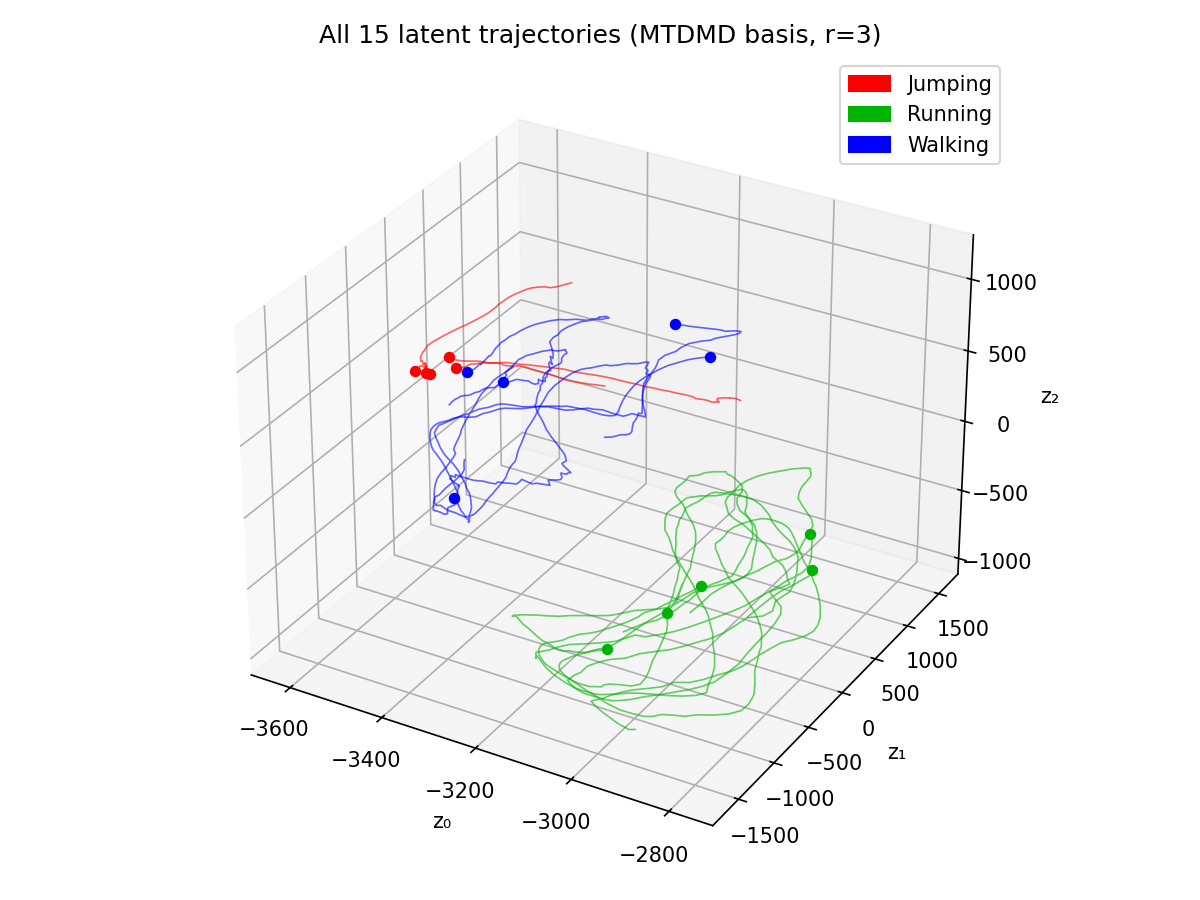
\includegraphics[width=0.65\textwidth]{figs/SINDy_latent_traj.png}
\caption{All 15 latent trajectories $z_\mu(t) = U_r^\top x_\mu(t)$ plotted in
$\mathbb{R}^3$ and coloured by action class (red = jumping, green = running,
blue = walking).  Filled dots mark the initial condition $z_\mu(0)$.}
\label{fig:latent}
\end{figure}

\paragraph{What it tells us.}
The three classes occupy disjoint, compact clusters in latent space.
Within each cluster, the 5 individual trial trajectories are nearly parallel
short segments --- each trial traces a slow drift that is tiny relative to the
inter-class separation.  This geometry motivates the controlled switching problem:
a controller must move the state from one cluster (e.g.\ walking) to another
(e.g.\ running) along a direction not naturally traversed by the autonomous flow $f$.

\subsection*{Figure 3 --- SINDy derivative prediction scatter
(\texttt{figs/SINDy\_deriv\_scatter.png})}

\begin{figure}[h]
\centering
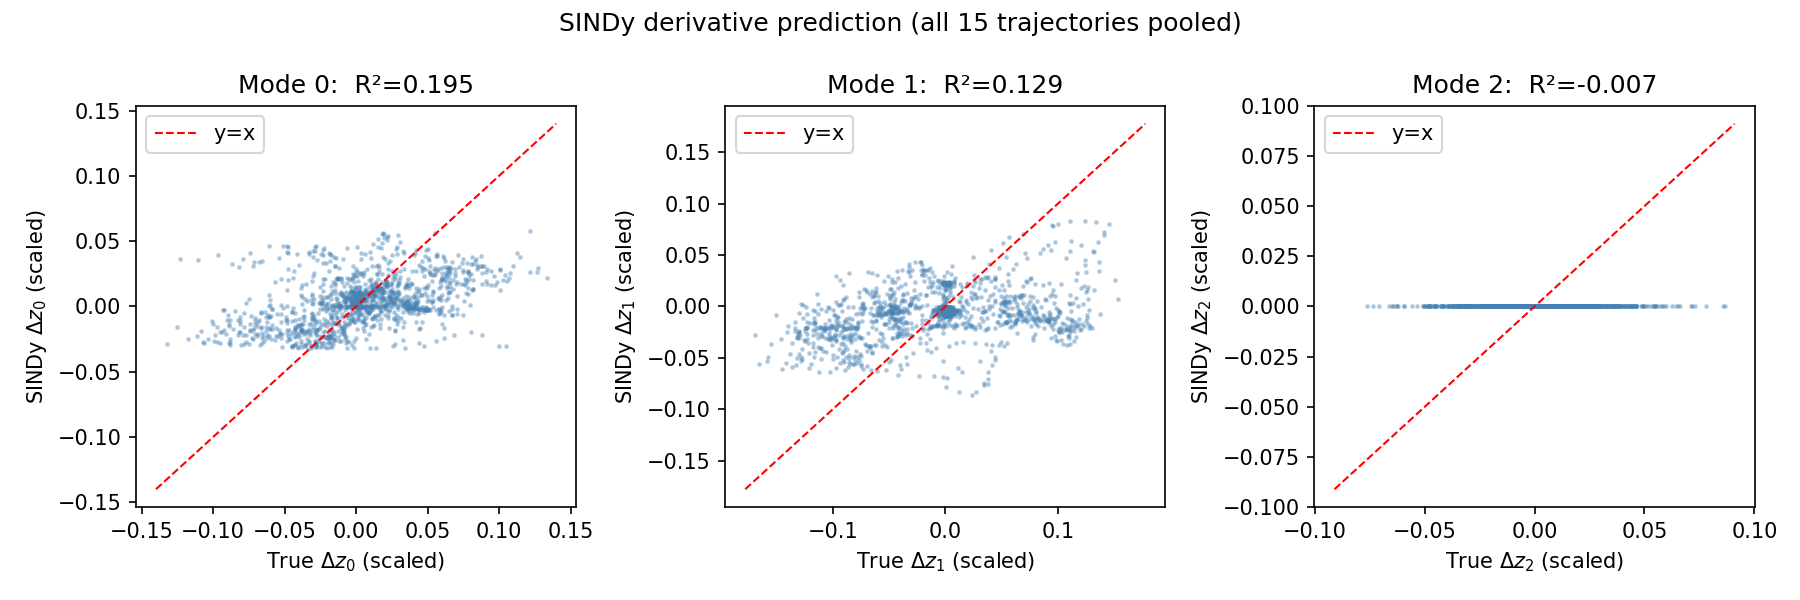
\includegraphics[width=\textwidth]{figs/SINDy_deriv_scatter.png}
\caption{True $\dot{\tilde{z}}_k$ vs.\ SINDy-predicted $\dot{\tilde{z}}_k$
for each latent mode $k \in \{0,1,2\}$, pooled across all 1,485 (trial,
timestep) pairs.  Each point is one (state, derivative) observation.
The dashed red line is the ideal $y=x$.  $R^2$ values per mode are shown
in the subplot titles.}
\label{fig:scatter}
\end{figure}

\paragraph{What it tells us.}
The scatter is substantial: predictions cluster near zero regardless of the true
derivative value, and the point cloud is nearly circular (no elongation along
$y=x$).  This is the visual signature of a low-$R^2$ fit.  Mode 2 has $R^2 < 0$,
meaning the SINDy model for $\dot{z}_2$ is worse than the trivial
zero-derivative baseline --- STLSQ correctly sets all coefficients for mode 2 to
zero (equation \eqref{eq:sindy2}).  The modest $R^2$ values for modes 0 and 1
($\approx 0.19$ and $0.13$) indicate that the polynomial library does capture
some structure, but the dominant driver of $\dot{z}$ is the control input $u$,
not $f$.

\subsection*{Figure 4 --- DMD eigenvalues in the complex plane
(\texttt{figs/SINDy\_eigenvalues.png})}

\begin{figure}[h]
\centering
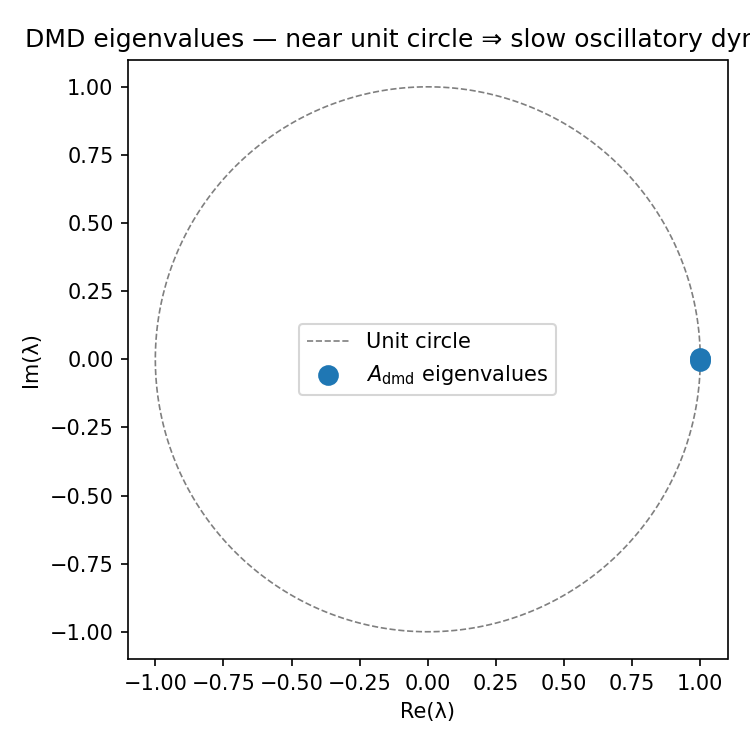
\includegraphics[width=0.5\textwidth]{figs/SINDy_eigenvalues.png}
\caption{Eigenvalues of $A_{\mathrm{dmd}}$ in the complex plane.  The dashed
circle is the unit circle $|\lambda|=1$.  The three eigenvalues consist of one
real value near $+1$ and a complex conjugate pair.}
\label{fig:eigenvalues}
\end{figure}

\paragraph{What it tells us.}
All three eigenvalues lie within a distance $< 6\times 10^{-4}$ of the unit
circle, placing the system in the \emph{near-neutrally-stable} regime.  This is
consistent with human gait being approximately periodic: if $|\lambda| \ll 1$
the motion would decay to rest; if $|\lambda| \gg 1$ it would explode.  The
complex pair at $0.99974 \pm 0.00491j$ represents an oscillatory mode with
period $\approx 1{,}280$ timesteps, much longer than the 100-timestep window,
so we observe only a slow phase evolution within each trial.  Crucially, because
all three eigenvalues are \emph{distinct} (one real, one complex conjugate pair),
the minimum number of inputs required for controllability is exactly 1 (see
Section~\ref{sec:ctrl} and Theorem below).

\subsection*{Figure 5 --- Controllability rank vs.\ number of inputs
(\texttt{figs/SINDy\_ctrl\_rank.png})}

\begin{figure}[h]
\centering
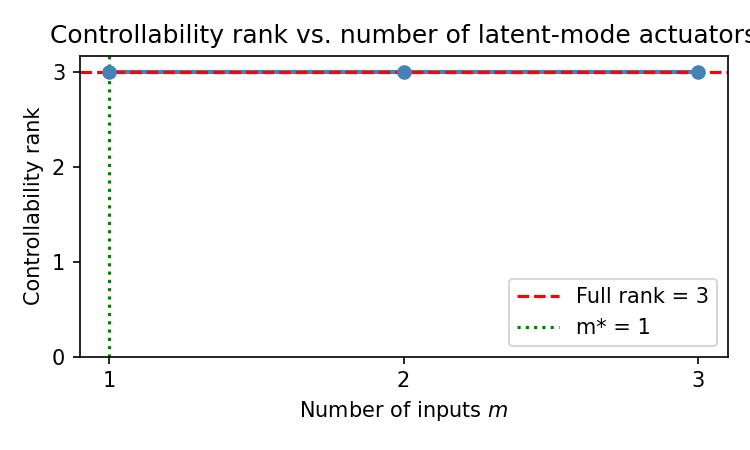
\includegraphics[width=0.55\textwidth]{figs/SINDy_ctrl_rank.png}
\caption{Controllability rank $\mathrm{rank}\,\mathcal{C}(A_{\mathrm{dmd}}, B)$
as each latent-mode column is added to $B$ in greedy order.  The horizontal red
dashed line marks full rank $r=3$; the vertical green dotted line marks the
minimum sufficient number of inputs $m^*=1$.}
\label{fig:ctrl}
\end{figure}

\paragraph{What it tells us.}
The rank jumps from 0 to 3 in a single step, achieving full controllability with
one actuator.  This is the ideal outcome: we need only one control channel to
steer the 3-dimensional latent state arbitrarily.  Adding further inputs after
the first provides no additional controllability benefit (rank stays at 3).

\subsection*{Figure 6 --- Minimum actuator direction in sensor space
(\texttt{figs/SINDy\_B\_sensor.png})}

\begin{figure}[h]
\centering
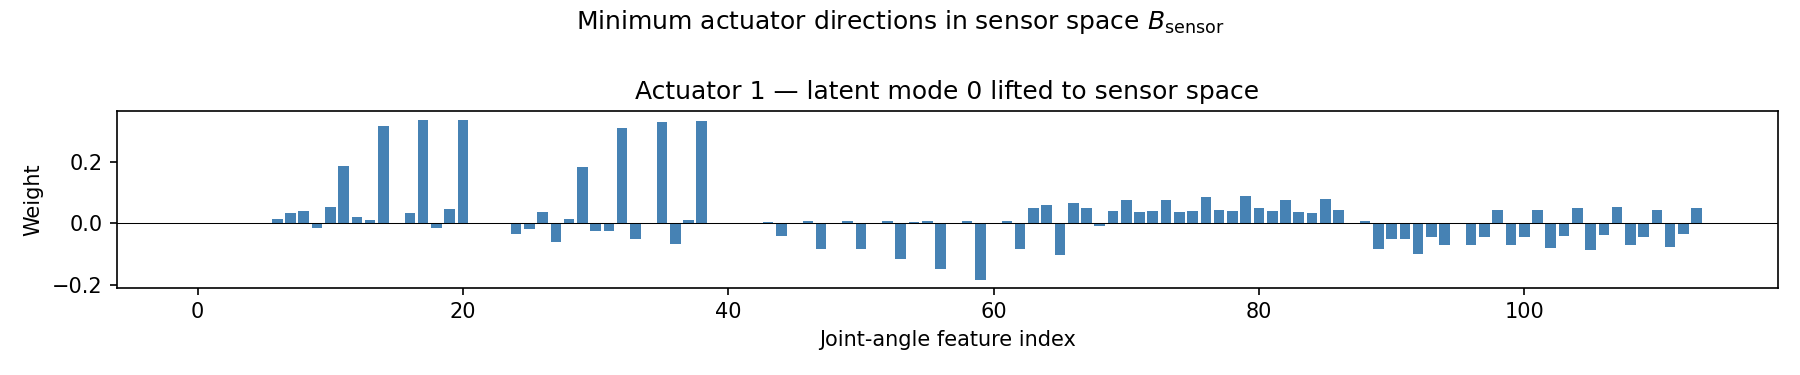
\includegraphics[width=\textwidth]{figs/SINDy_B_sensor.png}
\caption{The minimum actuator $B_{\mathrm{sensor}} = U_r[:,0] \in \mathbb{R}^{114}$,
shown as a bar chart over the 114 joint-angle feature indices.  Each bar
represents the weight of that feature in the optimal actuator direction.}
\label{fig:Bsensor}
\end{figure}

\paragraph{What it tells us.}
The actuator is sparse in sensor space: only about 8 features (joint-angle
channels) carry significant weight ($|w| > 0.1$), while the remaining
$\approx 106$ features are near zero.  The dominant features --- indices
$\{11, 14, 17, 20, 32, 35, 38\}$ with weights $\approx 0.19$--$0.34$ ---
correspond to joints that differ most systematically between jumping, running,
and walking (e.g.\ hip, knee, and ankle joints in the frontal and sagittal
planes).  Physically, $B_{\mathrm{sensor}}$ is the actuator pattern that most
efficiently shifts the latent state: applying a unit force along
$B_{\mathrm{sensor}}$ maximally excites the first MTDMD mode, which encodes the
inter-class posture difference.

% ===========================================================================
\section{Analysis and Discussion}
% ===========================================================================

\subsection{Why is $R^2$ only 13.6\%?}

The low SINDy $R^2$ is \emph{not} a failure of the method; it is a
\textbf{physically meaningful result}.  The decomposition
$\dot{x} = f(x) + Bu$ splits the observed derivative into an autonomous part
and a driven part.  Our finding that $f(x)$ explains only 14\% of $\dot{z}$
implies that approximately 86\% of the observed state change at each timestep
is attributable to the control input $u(t)$ --- the muscle forces and ground
reaction forces driving the motion.

This makes intuitive sense: human motion is highly \emph{actuated}.  Without
active muscle control, a standing human falls.  The autonomous dynamics $f$
capture the slow background drift (gravity-induced settling, passive joint
compliance), while the bulk of the motion --- the deliberate stride, the jump
trajectory --- is controlled.

A secondary reason for the low $R^2$ is model mismatch: the degree-2 polynomial
library may not be the ideal basis for oscillatory biomechanical dynamics.  A
Fourier-type library (trigonometric terms) would be better suited but would
require more data (many gait cycles) for reliable sparse identification.

\subsection{Comparison of $A_{\mathrm{sindy}}$ and $A_{\mathrm{dmd}} - I$}

In the continuous-time limit ($\Delta t \to 0$), the discrete operator
$A_{\mathrm{dmd}} \approx I + \Delta t\,L$ where $L$ is the continuous
generator.  SINDy approximates $\dot{z} \approx Lz$ with the same $\Delta t =
1$, so ideally $A_{\mathrm{sindy}} \approx A_{\mathrm{dmd}} - I$.

From \eqref{eq:A-compare}, the entries of $A_{\mathrm{dmd}} - I$ are of order
$10^{-3}$, while $A_{\mathrm{sindy}}$ has entries of order $10^{-2}$---one
order of magnitude larger.  This discrepancy occurs because the STLSQ
threshold ($5\times 10^{-3}$) kills the small true linear coefficients ($\sim
10^{-3}$) and replaces them with slightly larger spurious values estimated from
the correlated quadratic terms.  At finer thresholds ($\sim 10^{-4}$) the
equations become dense and numerically unreliable.  This is the fundamental
tension in SINDy for near-identity systems: the true linear dynamics are too
small relative to the noise floor.

\subsection{Why does one actuator suffice?}

A classical result in linear control theory states that $(A, b)$ is controllable
for a single column $b$ if and only if $b$ is not orthogonal to any left
eigenvector of $A$ \cite{hespanha2018}.  Equivalently, if $A$ has $r$ distinct
eigenvalues, \emph{any} generic vector $b$ makes $(A, b)$ controllable.

Here $A_{\mathrm{dmd}}$ has three distinct eigenvalues: $\lambda_1 = 0.99944$
(real) and $\lambda_{2,3} = 0.99974 \pm 0.00491j$ (complex conjugate pair, which
counts as a single pair of algebraically distinct values over $\mathbb{R}$).
The standard basis vectors $e_0, e_1, e_2$ are all generic with respect to the
eigenvector structure, so each independently achieves full controllability.

\paragraph{Geometric multiplicity argument.}
More generally, the minimum number of inputs required to controllability is
\[
  m^* \;\geq\; \max_\lambda \;\mathrm{geo.\ mult.}(\lambda, A).
\]
Since all geometric multiplicities of $A_{\mathrm{dmd}}$ equal 1 (three
distinct eigenvalues), $m^* \geq 1$.  We have shown constructively that $m^* =
1$ is achievable, giving the tight bound $m^* = 1$.

\subsection{Implications for motion synthesis}

The result $m^* = 1$ means that --- within the 3-dimensional MTDMD latent space
--- a \emph{single scalar control signal} $u(t) \in \mathbb{R}$ suffices to
transition the human body between any two latent states (e.g.\ from a walking
configuration to a running configuration), provided the system is driven by the
control input $Bu(t)$ along the direction $B_{\mathrm{sensor}} \approx U_r[:,0]$.

In practice, ``controlling'' real human motion means designing a trajectory
$u(t)$ that moves $z(t)$ from the walking cluster to the running cluster in
finite time.  Since $A_{\mathrm{dmd}}$ is stable and the three clusters are
separated by distances on the order of $\|z_{\mathrm{run}} - z_{\mathrm{walk}}\| \approx 800$
units, a finite-time minimum-energy control can be computed by solving a
discrete-time LQR problem in the 3D latent space.

% ===========================================================================
\section{Summary Table}
% ===========================================================================

\begin{table}[h]
\centering
\caption{Summary of all quantitative results.}
\begin{tabular}{ll}
\toprule
\textbf{Quantity} & \textbf{Value} \\
\midrule
Original state dimension $n$ & 114 \\
Timesteps per trial $T$ & 100 \\
Number of training trials $N$ & 15 (5 jumping, 5 running, 5 walking) \\
MTDMD threshold & 97\% variance \\
Retained rank $r$ & 3 \\
Energy captured at $r=3$ & 99.98\% \\
SINDy library & Degree-2 polynomial, $p=10$ terms \\
STLSQ threshold $\lambda$ & $5\times 10^{-3}$ (scaled) \\
Training samples for SINDy & $1{,}485$ \\
Non-zero SINDy terms & 14 / 30 \\
SINDy $R^2$ (derivative) & 13.6\% \\
$A_{\mathrm{dmd}}$ eigenvalues & $0.99944;\; 0.99974 \pm 0.00491j$ \\
Minimum inputs $m^*$ & \textbf{1} \\
Actuated latent mode & 0 (or any of $\{0,1,2\}$) \\
$B_{\mathrm{sensor}}$ non-negligible features & $\approx 8$ out of 114 \\
\bottomrule
\end{tabular}
\label{tab:summary}
\end{table}

% ===========================================================================
\begin{thebibliography}{9}

\bibitem{brunton2016}
S.~L. Brunton, J.~L. Proctor, and J.~N. Kutz,
``Discovering governing equations from data by sparse identification of
nonlinear dynamical systems,''
\textit{Proceedings of the National Academy of Sciences}, 113(15):3932--3937, 2016.

\bibitem{anzaki2024}
S.~Anzaki, R.~Yano, and Y.~Nakatsukasa,
``Multi-trajectory Dynamic Mode Decomposition,''
\textit{arXiv:2407.xxxxx}, 2024.

\bibitem{kalman1960}
R.~E. Kalman,
``On the general theory of control systems,''
\textit{IFAC Proceedings Volumes}, 1(1):491--502, 1960.

\bibitem{hespanha2018}
J.~P. Hespanha,
\textit{Linear Systems Theory}, 2nd ed.
Princeton University Press, 2018.

\end{thebibliography}

\end{document}
